\section{Philosophy and methods}
\label{sec:philosophy_and_methods}

% Q.
Why do we need a model that might enable us to observe the
creative process in the artistic outcome or practice e.g poems? Or,
how can we justify building such a model based on the outcomes of
creative practice i.e poems?

% A.

1. Because the originary and therefore the unpredetermined nature of
the creative process means that the post-fact outcome represents a
more accurate and objective evidence of it than the poet's attempt to
explain it as it happens.  According to Kant, the creation of a work
of art (e.g poetry) succeeds in exhibiting originality that is neither
predictable before it occurs nor traceable to prior rules
\cite{anderson1992role}.  So a creator discovers how and what he/she
is expressing through the creative process only in the course of doing
it. And we, as observers, are therefore only able to consider how a
creator selected and rejected various possibilities during the
creative process, by considering the creation after the fact and
within the finished whole.

2. Making a model of the creative process incorporates Dewey's ideas
that the content of the art form is not the same as the aesthetic
emotion expressed in it \cite[p. 35]{dewey2005art}. It is a reasonable
extrapolation from this notion to the idea that the content of an art
form represents and indicates an examination of how it was made.

% Q
If content does not represent conceit, metaphor or what
might be termed raw ingredients or some emotional spark felt the
artist, how can a new way of considering content result in a rigorous
and analytical study of the creative process?

% A
Examining the content of the poem is a way of examining what it tells
us about the drivers propelling it through its own making and how it
stands as observer of its own process.  ``The painter does not paint;
he watches himself paint'' \cite[p. 7]{collingwood1958principles} ``In a poem, objective
material becomes the content and the matter of the emotion and not
just its evocative occasion'' \cite[p. 69]{dewey2005art}.

% Q
What is the central plank to this way of linking the outcome (or
creative practice) with the creative process?

% A
The idea that creation involves an exploration and expression of an
aesthetic emotion and that both these can be charted or mapped in the
creative outcome (the poem).

% Q
What is being expressed?

% A
The artist, in the course of creating, is involved in something
Collingwood referred to as ``the expression of aeasthetic emotion''
\cite[p. 117]{collingwood1958principles}. In Part I of his Principles
of Art, Collingwood suggests that the creative process takes place in
stages. These are not necessarily chronological but present as a
manifestation during creation that is visible in its outcome.

% Q
What do we mean by the ``expression of an aesthetic emotion''?

% A
I refer you to Collingwood and also to Benedetto Croce here for a
combined definition of how an aesthetic emotion is expressed - An
aesthetic emotion is expressed via a total imaginative activity. This
is taken from Collingwood's Principles (1938) and Croce's Aesthetic
(1902).  It is be relevant to the analysis of the poems that Croce's
  Aesthetic defined intuition as ``the non-divisible expression of
  sympathy'' \cite[pp. 171--193]{kemp2003croce}.

% Q
What are the steps, stages or aspects of the creative process?
[``Aspect'' is my preferred term as it removes us from chronology and
  the implication that all these must be present all the time. Think
  instead that they can be ``evidenced''].

% A
Collingwood describes the initial stages of expression as
``oppression''; as something that happens to the artist during his/her
exploration of the creative process and, unexpressed, this produces
feelings that are oppressive and which Dewey described as
``disturbance'' and which Anderson and Hausman see as a ``colouring''.

% Q
What happens to this oppression or disturbance?

% A
The artist becomes conscious of it and starts to explore his/her own
expression of it. This takes place as an intuited feeling (as
described by Croce). This gives rise to a new feeling of alleviation
or easement. That reference to novelty is crucial. If something is
new, it cannot be predetermined.

% Q
What do we mean by ``aesthetic emotion''?

% A
PG Whitehouse on Dewey's Art as Experience suggests that Dewey joins
Collingwood in separating aesthetic emotion from any notion that
inspiration can be considered as something like raw materials. This
fits in with our view of content as representational (and certainly
indicative) of the creative process of the poet. So an emotion is
aesthetic when it ``adheres to an object formed by an expressive act''
\cite[pp. 149--156]{whitehouse1978meaning}.  Or better still, ``the art
object does not have emotion for its significant content\ldots.Emotion
is a conscious sign of a break, actual or impending. It belongs to the
self that is concerned in the movement of events toward an issue that
is desired or disliked'' \cite[p. 14]{dewey2005art}.

% Q
What do we mean by experience?

% A
``An unanalysed whole in a situation, having a pervasive quality in
which the self finds itself'' \cite[p. 3]{zeltner1975john}.

% Q
In what way (in what phases/stages/aspects) can we see the artist
experiencing aesthetic emotion in the making of his/her art?

% A
In a study of Collngwood's theory of the expression of aesthetic
emotion, Doug Anderson and Carl Hausman refine ideas on how we might
see this and specifically how this relates to our way of studying
process through practice \cite[pp. 299-305]{anderson1992role}:

\begin{quote}
Aesthetic emotion\ldots  response\ldots  artist's decision on components of expression\ldots feeling of easement plus a simultaneous emerging of a unique imaginative expression\ldots alleviation\ldots consciousness\ldots specific to converting psychical emotion\ldots unique aesthetic experience 
\end{quote}

% Q
What is psychical emotion?

% A
The agent (through expression) discovers him/herself to have been
feeling independently of expressing it. [The emotion of consciousness
  is where an agent only feels at all in so far as he/she thus
  expresses it].

% Q
How is easement understood to be unique/originary?

\begin{quote}
Aesthetic emotion\ldots attends to successful expression\ldots contributes integrally to what is expressed in its specificity\ldots functions as individualsed clue\ldots at each crucial moment of a developing imaginative experience
\end{quote}

Conclusion: The poem is a work of progress, rather than a work in
progress.

Although it is beyond the scope of the current work to trace these
connections, we will remark that this view is connected with the
Bergson genre of philosophy, running to Mead who offers a generalised
view of the social, to Bakhtin who develops the notion of dialogue in
a broad metalinguistic frame, and to Deleuze who develops a processual
ontology based on the idea of difference \cite{bergson1983creative,
  mead1932philosophy, bakhtin1984problems, deleuze1994difference}.
These perspectives are relevant to the interest we take here in
emergence, polyvocality, and learning by specifying and engaging with
problems.

\subsection{Methods: ``What are the proposed `lab rats'?''}
\label{sec:methods}

\begin{figure}
\resizebox{\columnwidth}{!}{%
%% For final:
\begin{tikzpicture}
%  \draw[thick] (4,0) node[below={2cm}] {\emph{A.~``mere generation''}}
%                     pic[red, -latex]{darc=100:270:1.3cm:Chicken:Lay:2.4cm:3cm}
%                     pic[red, -latex]{uarc=280:450:1.3cm:Egg:Hatch:1cm:.1cm};
%
  \draw[thick] (4.0,0) node[below={2cm},align=center] {\emph{A.~how to become a writer\footnotemark}}
                      pic[red, -latex]{darc=100:270:1.3cm:{}:{Write for 8 hours a day}:1cm:.3cm}
                      pic[red, -latex]{uarc=280:450:1.3cm:{}:{Read for 8 hours a day}:1cm:.3cm};
%
  \draw[thick](8.5,0) node[below={2cm}] {\emph{B.~``the Other''}}
                     pic[red, -latex]{darc=100:270:1.3cm:Statement:Speak:2.1cm:2.6cm}
                     pic[red, -latex]{uarc=280:450:1.3cm:Response:{Listens and interprets}:.2cm:.1cm};

%  \draw[thick] (4,-5.5) node[below={2.2cm}] {\emph{D.~learning by doing}}
%                        pic[red, -latex]{darc=100:240:1.5cm:Poet:Write:3cm:2.7cm}
%                        pic[red, -latex]{rarc=250:320:1.5cm:Poem:Responds:1cm:.5cm}
%                        pic[red, -latex]{uarc=330:450:1.5cm:Context:Speaks:1cm:.1cm};
%
%
  \draw[thick] (13,0) node[below={2cm}] {\emph{C.~proto-workshop}}
                        pic[red, -latex]{larc=100:180:1.3cm:Poet:Writes:1cm:.2cm}
                        pic[red, -latex]{rarc=190:270:1.3cm:Poem:Responds:1cm:.4cm}
                        pic[red, -latex]{rarc=280:360:1.3cm:Context:Speaks:.7cm:.7cm}
                        pic[red, -latex]{larc=370:450:1.3cm:Reader:Responds:.8cm:.2cm};

%  \draw[thick] (13,-5.5) node[below={2.2cm}] {\emph{F.~how computers work}}
%                       pic[red, -latex]{darc=100:180:1.5cm:{}:Print:1.5cm:1.4cm}
%                       pic[red, -latex]{rarc=190:270:1.5cm:{}:Loop:1cm:1.4cm}
%                       pic[red, -latex]{rarc=280:360:1.5cm:{}:Read:1cm:1.4cm}
%                       pic[red, -latex]{larc=370:450:1.5cm:{}:Eval:1.4cm:.2cm};
% Note:
% controls at end: offset of outer text, followed by offset of inner text
\end{tikzpicture}

%% For quick compiling
% 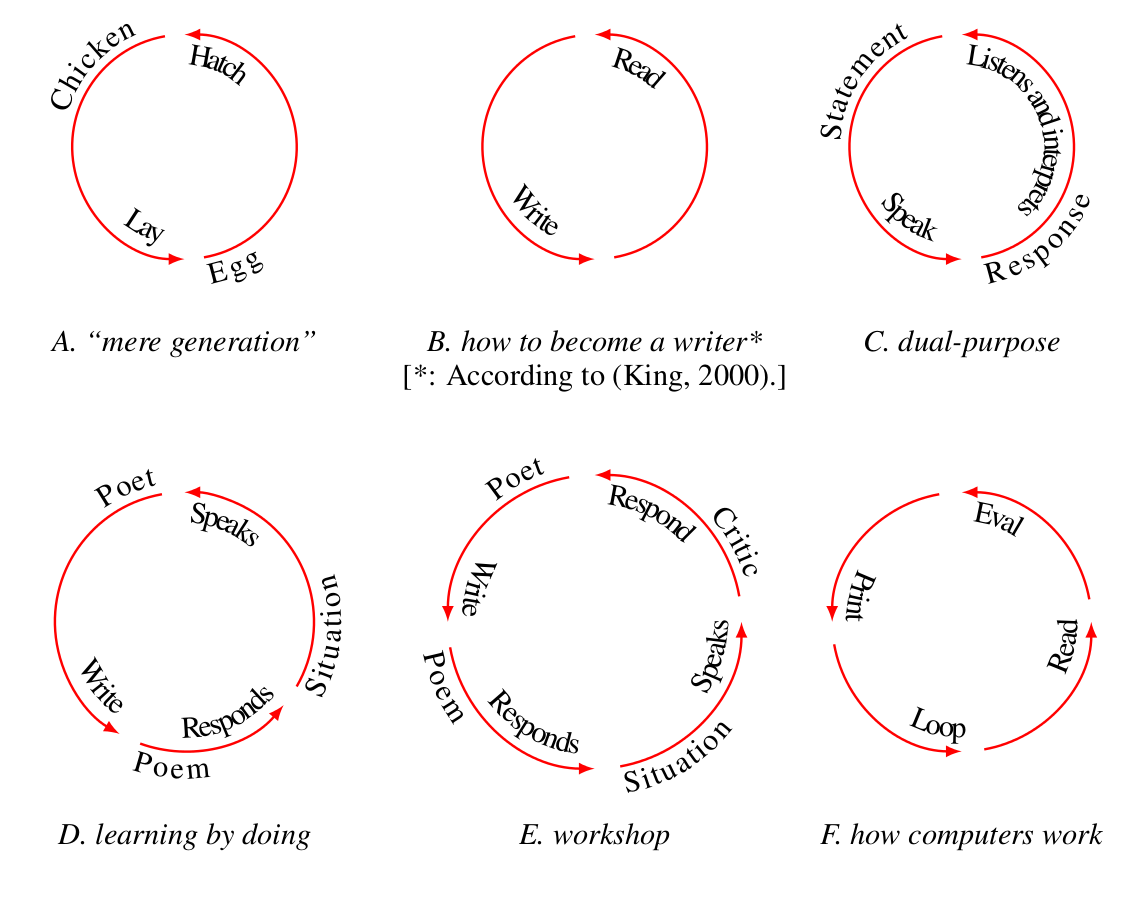
\includegraphics{figures/cycles_shortcut}
}

\caption{(A) gives a simple recipe for the growth and
development of a writer;
(B) \emph{response} always has dimensions that goes beyond the
utterance that is overheard;
(C) adds a \emph{reader} who shares the context with the writer and responds.%, and who responds to this context particularly as it is expressed through the poem
\label{fig:cycles}}
\end{figure}


There are many possible places for a ``dialogical'' intervention
within the writing process; see Figure \ref{fig:cycles}.  Figure
\ref{fig:cycles}(A) shows the standard chicken-and-egg problem,
designed to provoke questions about \emph{evolution}; 1(B) shows an
analogous picture that gives a simple recipe for the growth and
development of a writer; 1(C) is a formally similar diagram that
squares up to the metalinguistic features of the situation, showing
that a \emph{response} (which may be verbal, visceral, physical or
something else) always has dimensions that goes beyond the utterance
that is overheard; 1(D) examines in further detail what happens when
someone \emph{writes} -- namely, writing as a response to a situation
that may allow the writer to make sense of this situation; 1(E) adds a
\emph{critic} who responds to the situation, particularly as it is
expressed through and enhanced by the poem; 1(F) shows that this
scenario is not as unfamiliar to computer programmers as it might
otherwise sound -- consider that the ``Eval'' phase in a
Read-Eval-Print loop can be interrupted with a debugger to fine-tune
program operation.

Our ``lab rats'' are, accordingly, not poems -- which could, after
all, be developed through ``mere generation'' -- but are, rather,
\emph{instances of reading and responding to poetry}.  This may take
place within a formal ``workshop'' context or they may take place in
smaller-scale experiments where a computer system reads and responds
to other poets.  Naturally, such responses can also be more or less
``canned'' (as with Michael Cook's humorously nonspecific
AppreciationBot), so the question becomes what constitutes an
authentic, interesting, or useful response, and how will these be
developed?  The idea of responses is also useful at the micro-level,
as will be made clear in the following section.  We focus here on the
big picture of staging a encounter, supported by preliminary
implementation work.

%%% Local Variables: 
%%% mode: latex
%%% TeX-master: "poetryICCC"
%%% End: 
